\chapter{页表和内存管理}\label{ch:page-tables-and-memory-management}

\section{内存管理概述}\label{sec:3-memory-management-overview}

内存管理（Memory Management）指的是对物理内存（Physical
Memory）及虚拟地址空间（Virtual Address
Space，VAS）进行的分配和回收操作。要保证内存管理的安全性，硬件上的支持是必要的。RME 操作系统的内存管理支持内存保护单元（Memory
Protection Unit，MPU）环境和内存管理单元（Memory Management
Unit，MMU）环境，并且它们被抽象成了相同的页表数据结构。本章中所用到的术语的定义如下：

\begin{xltabular}{\textwidth}{@{}>{\hsize=0.7749\hsize\raggedright\arraybackslash}X>{\hsize=1.2251\hsize\raggedright\arraybackslash}X@{}}
\caption{页目录术语定义}\label{tab:3-1-page-directory-terminology}\\
\toprule
术语 & 定义\tabularnewline
\endfirsthead
\toprule
术语 & 定义\tabularnewline
\midrule
\endhead
\bottomrule
\endlastfoot
页表（Page Table，PT） &
指的是整个页表本身，包括了顶层页目录和中间的各个级别的页目录，是一棵地址树的总称。\tabularnewline
页目录（Page Directory，PD） &
指的是页表中的一级，其中最顶层的一级被称为顶层页目录。\tabularnewline
页表项（Page Entry，PE） &
指的是页目录表格中的一项，它可能指向一个页，也可能指向下一级页目录。其中，我们把指向页的叫做末端页表项（Page
Terminal Entry，PTE），把指向下一级页目录的叫做中间页表项（Page
Intermediate Entry，PIE）。\tabularnewline
\end{xltabular}

\section{页表的操作和结构}\label{sec:3-page-table-operations-and-structure}

页表是由一系列页目录组成的多层基数树（Radix Trie/Radix
Tree）结构。页目录的每一个槽位都被固定为一个机器字的长度。页目录中的每一个槽位都可以放置以下三种数据之一：下级页目录物理地址、页表项物理地址及属性或空页表项。如果存放的是下级页目录物理地址，那么代表此处有一个下级页目录，该部分虚拟地址的映射关系要查询该页目录决定；如果存放的是页表项物理地址及属性，则代表此虚拟地址处有一个页表项被映射，并且可以得知该页的访问属性；如果存放的是空页表项，那么则说明这个虚拟地址处没有任何东西被映射。在 RME 中，页表是需要用户手动构造的，这和 Composite 等一系列微内核的解决方法是一致的\hyperref[cite:3-1]{{[}1{]}}。

\subsection{内核内存和用户内存}\label{subsec:3-kernel-memory-and-user-memory}

RME 的系统内存被分为两部分：一部分是内核内存，一部分是用户内存。和 Composite、L4 等微内核不同，在 RME 系统中，内核内存映射是在一开始就完全建立\footnote{静态或半静态分配}的，并且不可修改。这使得 RME 完全不需要内存动态类型机制\footnote{这种机制被Composite、seL4等系统采用\hyperref[cite:3-1]{{[}1{]}}\hyperref[cite:3-3]{{[}3{]}}。在 RME 中它其实也可以被受信任的用户态服务器实现}，而且内存管理系统完全可并行化，同时彻底免去了内核内存内容泄露的可能。对于MMU环境，在创建顶层页目录时，系统会将在启动时就创建好的内核页目录映射到顶层页目录之内；对于MPU环境，由于内核态通常都有对整个内存的访问权限，因此在所有页目录中我们只需要用户页就可以了\footnote{某些架构（如 Tricore 等）需要保留一个或者多个MPU寄存器组给内核态，但是这些页并不会反映在页表中}。

在系统启动时，所有的用户物理内存页都被加入了启动进程（Init）的页表之中。在这种添加结束之后，通常而言不再允许系统凭空地创造物理内存页框，除非使用自定义内核调用\footnote{见第~\ref{sec:8-kernel-call-implementation-overview}~节}。在创建新进程时，新进程的页表的页表项是必须从其他进程处添加过来的。在添加时，可以指定这个页的访问属性，并且所指定的访问属性一定要是父页面的访问属性的一个子集。RME 系统中，页访问的标准属性如下表：

\begin{xltabular}{\textwidth}{@{}>{\hsize=0.5857\hsize\raggedright\arraybackslash}X>{\hsize=0.7809\hsize\raggedright\arraybackslash}X>{\hsize=1.6334\hsize\raggedright\arraybackslash}X@{}}
\caption{页访问的标准属性}\label{tab:3-2-standard-page-access-attributes}\\
\toprule
名称 & 标识符 & 意义\tabularnewline
\endfirsthead
\toprule
名称 & 标识符 & 意义\tabularnewline
\midrule
\endhead
\bottomrule
\endlastfoot
可读 & RME\_PGT\_READ & 这个页面是可读取的。\tabularnewline
可写 & RME\_PGT\_WRITE & 这个页面是可写入的。\tabularnewline
可执行 & RME\_PGT\_EXECUTE &
这个页面的是可作为代码执行的。\tabularnewline
可缓存 & RME\_PGT\_CACHE & 这个页面的内容可以被缓存。\tabularnewline
可缓冲 & RME\_PGT\_BUFFER & 这个页面的写入可以被缓冲。\tabularnewline
静态 & RME\_PGT\_STATIC &
这个页面是总被映射的静态页。这意味着，MPU环境下或在手动更新TLB的MMU环境下，这个页总是被映射，而非等到缺页中断来临时映射。\tabularnewline
\end{xltabular}

值得注意的是，在某些架构中，上面的某些位可能不会全部都具有意义。比如，对于绝大多数自动更新快表（Trans
Look-aside
Buffer，TLB）的MMU环境，静态属性是没有意义的；对于某些架构，读和写是一起实现的，因此不具有分立的读写控制。

为了实现用户态对在创建内核对象时对内核内存的管理，系统中的内核对象使用一个内核对象登记表进行管理。内核对象登记表是一个位图，里面存储了内核对象对于虚拟地址的占用。这个位图保证了在同一段内核虚拟地址上，不可能同时存在两个内核对象。

为了防止某些有权创建内核对象的系统组件在出错或被入侵时大量创建内核对象从而耗尽内核内存，发动拒绝服务（Denial
of
Service，DoS）攻击，因此引入了内核内存权能来管理内核内存。内核内存权能的概念参考了 Fiasco.OC 的内核对象工厂（Factory）\hyperref[cite:3-4]{{[}4{]}}。在创建任何一个内核对象时，都需要内核内存权能；该内核内存权能标志了允许用来创建内核对象的内核虚拟内存地址范围，以及允许在这段内存上创建哪些对象。只有当被创建的内核对象完全落在这个范围之内，并且该内核内存权能的标志位允许创建该种对象时，创建操作才能够被继续进行，否则将返回一个错误，从而限制某些被感染的恶意内核组件发起拒绝服务攻击。

\subsection{页目录的属性}\label{subsec:3-page-directory-attributes}

在 RME 操作系统中，页目录有四个属性。这四个属性唯一决定了页目录的状态。我们下面将分别介绍这四种属性。

\subsubsection{映射起始地址}\label{subsubsec:3-mapping-base-address}

映射起始地址指该层页目录开始映射的虚拟地址。这个页目录的第一个槽位的物理内存或者映射的二级页表的起始地址，就是这个虚拟地址。当我们试图把一个更底层的页目录映射到某高层次页目录的某位置时，我们可能需要检查底层的虚拟地址是否和高层的虚拟地址匹配，从而决定能否进行该映射。当然，这个检查仅仅在使用MPU的系统中是必须的。在使用MMU的系统中，由于一个页目录经常会被映射进不同的页目录的不同位置，这个检查可以被配置为不进行，此时映射起始地址一项无效，此时也无法使用路径压缩页表（Path-Compressed
Page
Table，PCPT）格式\footnote{MMU系统一般也不支持此格式}。有关路径压缩页表格式、MPU系统和MMU系统的差别请见后续章节。

\subsubsection{顶层页目录标志}\label{subsubsec:3-top-level-page-directory-flag}

标志着该页目录为最顶层的页目录。只有最顶层的页目录才可以被用来创建进程。

\subsubsection{页目录大小级数}\label{subsubsec:3-page-directory-size-order}

页目录大小级数决定了页目录每个槽位代表的虚拟地址的大小。如果某页目录的大小级数为12，那么就意味着该页目录中的每个槽位都对应2\textsuperscript{12}=4096字节大小的一个页。

\subsubsection{页目录数量级数}\label{subsubsec:3-page-directory-number-order}

页目录数量级数决定了页目录中的槽位数量。如果某页目录的数量级数为10，那么就意味着该页目录中一共有2\textsuperscript{10}=1024个槽位。

\subsection{页目录的基本操作}\label{subsec:3-basic-page-directory-operations}

在页目录上一共有六种基本操作，分别如下：

\begin{xltabular}{\textwidth}{@{}>{\hsize=0.8417\hsize\raggedright\arraybackslash}X>{\hsize=1.1583\hsize\raggedright\arraybackslash}X@{}}
\caption{页目录的基本操作}\label{tab:3-3-basic-page-directory-operations}\\
\toprule
操作 & 含义\tabularnewline
\endfirsthead
\toprule
操作 & 含义\tabularnewline
\midrule
\endhead
\bottomrule
\endlastfoot
创建页目录（Create） & 创建一个新的空页目录。\tabularnewline
删除页目录（Delete） & 删除一个页目录。\tabularnewline
映射内存页（Add） &
添加一个物理内存页到页目录的某虚拟地址处。\tabularnewline
移除内存页（Remove） &
删除页目录某虚拟地址处的一个物理内存页。\tabularnewline
构造页目录（Construct） &
添加一个子页目录到父页目录的某虚拟地址处。\tabularnewline
析构页目录（Destruct） &
删除父页目录某虚拟地址处映射的一个子页目录。\tabularnewline
\end{xltabular}

这六种操作在MPU和MMU上的实现是很不同的，也有不同的限制。请参看下面两节的解释以理解具体差别。

\subsection{内存管理单元下正常多级页表的实现}\label{subsec:3-normal-multilevel-page-table-under-mmu}

对于内存管理单元，页目录的实现是非常简单的，就是一个简单的线性表。比如，对于 x86-64 的页表，其第一级页目录（PML4）是固定的 512 个槽位，每个槽位代表2\textsuperscript{39}字节；第二级页目录（PDP）也是固定的 512 个槽位，每个槽位代表2\textsuperscript{30}字节；第三级页目录（PGD）也是固定的 512 个槽位，每个槽位代表2\textsuperscript{21}字节；第四级页目录（PTE）也是固定的 512 个槽位，每个槽位代表2\textsuperscript{12}字节。这四级页目录组成的基数树就是整个页表，如下图所示。其中，蓝色槽位代表指向子页目录的条目，而灰色槽位则代表被映射的页。此外，这些页目录的内存起始地址都应该对齐到4kB，这样它们都正好占据一个页。

\begin{figure}[htbp]
    \centering
    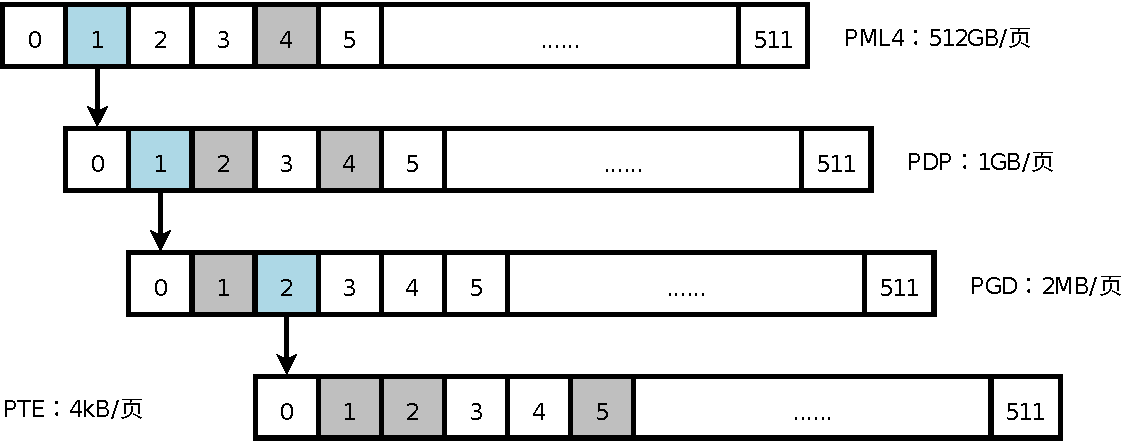
\includegraphics[width=0.72\textwidth]{Figure/image8.pdf}
    \caption{正常多级页表的例子}
    \label{fig:3-1-normal-multilevel-page-table-example}
\end{figure}

此外，如果允许一个页目录被构造进更高级页目录的任意虚拟地址槽位\footnote{只要大小和数量级数合适}，那么我们可以将内核配置为不检查起始虚拟地址是否合适。此时，我们使用的是正常多级页表，无需实现路径压缩。

由于处理器具备直接处理页表的硬件，因此我们不需要专门针对处理器生成页表元数据。但是需要注意，调用页表创建功能时，创建的页表应该合乎硬件页表查找机制的要求。对于那些纯软件填充TLB的MMU，则没有这个要求了，可以随意创建逻辑上符合页表形式的树结构，也可以把它们看成是基于区域的MMU，按照\ref{subsec:3-path-compressed-page-table-under-mpu}
所述的办法解决。

一些常见的MMU的特性如下：

\begin{xltabular}{\textwidth}{@{}>{\hsize=0.8979\hsize\raggedright\arraybackslash}X>{\hsize=0.6440\hsize\raggedright\arraybackslash}X>{\hsize=1.4399\hsize\raggedright\arraybackslash}X>{\hsize=1.0182\hsize\raggedright\arraybackslash}X@{}}
\caption{常见MMU的特性}\label{tab:3-4-common-mmu-features}\\
\toprule
处理器 & 页表级数 & 页大小 & 其他特性\tabularnewline
\endfirsthead
\toprule
处理器 & 页表级数 & 页大小 & 其他特性\tabularnewline
\midrule
\endhead
\bottomrule
\endlastfoot
ARM926EJ-S & 2或3级 & 1MB，64kB，4kB，1kB &
TLB部分表项手动锁定\tabularnewline
x86-64（AMD64） & 3级 & 1GB，2MB，4kB &
额外的段式内存管理单元\tabularnewline
Itanium（IA-64） & 4级 & 256MB，16MB，4MB，1MB，256kB，64kB，8kB，4kB &
可部分手动填充的TLB\tabularnewline
e200（PowerPC） & 不适用 & 1kB-4GB的所有2的次方 &
纯软件填充的TLB\tabularnewline
ARMv7-A（32-bit） & 2或3级 & 4kB，64kB，1MB，16MB &
TLB部分表项手动锁定\tabularnewline
ARMv8-M（64-bit） & 3或4级 & 4kB，16kB，64kB &
虚拟化下可选的2阶转换\tabularnewline
MIPS64 & 不适用 & 1kB-256MB的所有4的次方 &
纯软件填充的TLB\tabularnewline
TMS320C66X & 不适用 & 4kB-4GB的所有2的次方 &
纯软件填充的TLB\tabularnewline
\end{xltabular}

\subsection{内存保护单元下路径压缩页表的实现}\label{subsec:3-path-compressed-page-table-under-mpu}

在内存保护单元\footnote{或者手动填充的、基于区域的内存管理单元，下同}下，处理器往往不能直接识别多层的页表。这使得我们必须从页表生成MPU元数据用来在进程切换时高效地设置MPU。而且，在MPU环境下，还有如下的几个特点：

\begin{enumerate}
\def\labelenumi{\arabic{enumi}.}
\item
  MPU的区域个数往往是有限的，比如ARMv7-M有最多16个区域，每个区域又可以划分为8个子区域。因此，我们在一个进程中最多只能允许同时映射128个区域，而且这些区域还要满足一系列地址对齐等苛刻条件。因此，我们可以考虑把页分成两类，一类是静态页，它们总是被映射，要求可预测性的应用可以使用它们，静态页的最大数目就是处理器允许的最大MPU区域个数；另一类是动态页，它们只在使用时被映射，不保证在任何时候都被映射，动态页的最大数目是没有限制的。如果访问到了一个当前没有映射的动态页，那么处理器会进入缺页中断，然后我们手动查找页表来将该动态页加入MPU元数据，此时如果MPU区域不够可能会替换掉其他的动态页\hyperref[cite:3-2]{{[}2{]}}。
\item
  在一个页表里面，往往只有一两项是存在的。对于使用MPU的微控制器而言，维持多级页表的存在是没有必要的资源浪费，因此应该想办法对页表进行压缩。压缩页表和通常的页表相比，同一个页目录的不同中间页表项转换的地址位数可以是不同的。比如，在某个虚拟地址处，有一个很小的页，我们需要把它添加进访问范围。对于通常的页表，我们需要多级中间页目录，然后在最后一级页目录处，将这个页添加进去。而对于压缩页表，我们只要一级页目录就足以寻址该页。我们可以注明这个页目录的起始地址，数量级数和大小级数，然后直接将其构造进上级页目录中。当然，此时我们要求这一级页表所表示的虚拟地址范围落在上一级页目录的相应页表项允许的虚拟地址范围内。上述情况有一个例外：当架构实际上具备基于区域的MMU单元时，我们通常不使用路径压缩页表。
\item
  MPU不能进行物理地址到虚拟地址的转换。因此，虚拟地址总是等于物理地址的。这使得我们在映射页时必须检查页的映射地址是否等于物理地址。
\item
  由于我们需要MPU元数据来加速MPU填充，因此当我们修改任何一级页目录时，我们都必须维持元数据和页表的一致性。不维持这种一致性也是可以的，不过如果如此我们就只能通过缺页中断来更新元数据。而通过缺页中断来更新元数据并不总是可能的：部分架构在部分或全部情况下不提供缺页地址等关键信息。关于这种做法的详细信息请参看\ref{subsubsec:3-update-mpu-metadata-on-page-fault}
  。

  一个ARMv7-M上的路径压缩页表的例子如下图所示。绿色槽位代表路径压缩的指向子页目录的条目，蓝色槽位代表非路径压缩的指向子页目录的条目，而灰色槽位则代表被映射的页。各级页表前面的十六进制数代表了该页表的起始映射地址。

\begin{figure}[htbp]
    \centering
    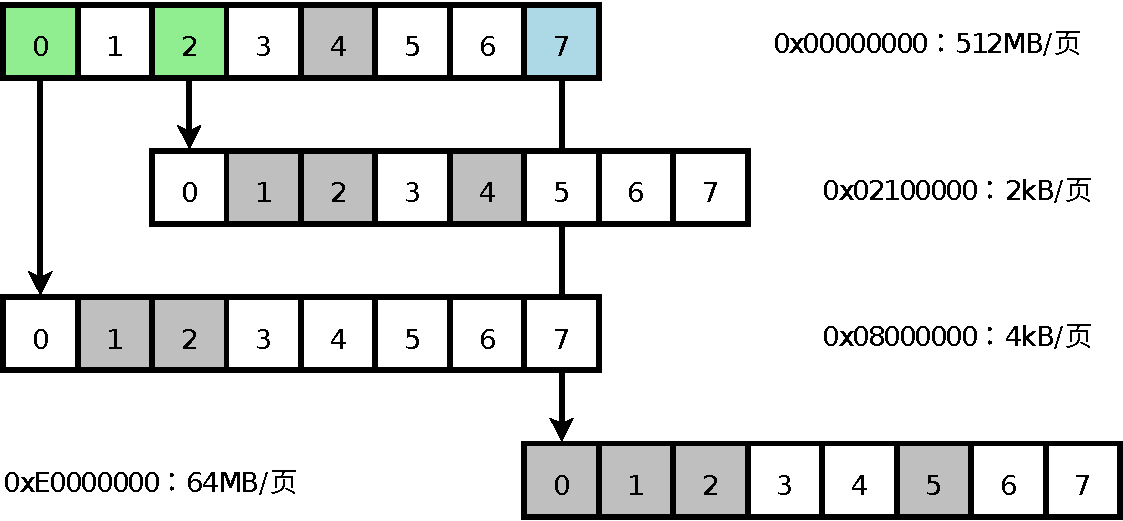
\includegraphics[width=0.72\textwidth]{Figure/image9.pdf}
    \caption{路径压缩页表的例子}
    \label{fig:3-2-path-compressed-page-table-example}
\end{figure}

  一些常见的MPU的特性如下：
\end{enumerate}

\begin{xltabular}{\textwidth}{@{}>{\hsize=1.0901\hsize\raggedright\arraybackslash}X>{\hsize=0.8740\hsize\raggedright\arraybackslash}X>{\hsize=1.1654\hsize\raggedright\arraybackslash}X>{\hsize=0.8740\hsize\raggedright\arraybackslash}X>{\hsize=0.9663\hsize\raggedright\arraybackslash}X>{\hsize=1.0301\hsize\raggedright\arraybackslash}X@{}}
\caption{常见MPU的特性}\label{tab:3-5-common-mpu-features}\\
\toprule
处理器 & 区域数量 & 区域组织 & 大小范围 & 对齐要求 &
其他特性\tabularnewline
\endfirsthead
\toprule
处理器 & 区域数量 & 区域组织 & 大小范围 & 对齐要求 &
其他特性\tabularnewline
\midrule
\endhead
\bottomrule
\endlastfoot
ARM v6-M & 0到16个 & 统一组织 & 128B-4GB & 对齐到大小 &
8个子区域\tabularnewline
ARM v7-M & 0到16个 & 统一组织 & 128B-4GB & 对齐到大小 &
8个子区域\tabularnewline
ARM v8-M & 0到16个 & 统一组织 & 128B-4GB & 无 & 无\tabularnewline
Tensilica L106 & 16或32个 & 统一组织 & 4kB-1GB & 无 & 无\tabularnewline
MIPS M14k & 1到16个 & 统一组织 & 任意 & 无 & 可锁定为只读\tabularnewline
PowerPC e200z4 & 32个 & 代码/数据各16个 & 任意 & 无 & 无\tabularnewline
AVR32 & 8个 & 统一组织 & 4kB-4GB & 对齐到大小 &
16个子区域\tabularnewline
MSP430FRXX & 3个 & 统一组织 & 任意 & 无 & 三段分段式\tabularnewline
Coldfire-MCF & 4个 & 代码/数据各2个 & 16MB-4GB & 对齐到大小 &
无\tabularnewline
RISC-V & 0到16个 & 统一组织 & 4B-4GB & 对齐到大小 &
也可对齐到字\tabularnewline
\end{xltabular}

综上所述，对于MPU下页表的实现，常见的有以下两种形式：

\subsubsection{更新页表时立即更新MPU元数据}\label{subsubsec:3-update-mpu-metadata-immediately}

这种做法仅仅把MPU元数据放置在顶层页目录中，而且要求构造时从顶层构造起。如果任何一级页目录没有顶层页目录，自己也不是顶层页目录，那么就无法构造子页目录到这个页目录之内。此外，任意两个页表都不能共享页目录或页目录树。这种实现的制约如下：

\begin{xltabular}{\textwidth}{@{}>{\hsize=0.5941\hsize\raggedright\arraybackslash}X>{\hsize=1.4059\hsize\raggedright\arraybackslash}X@{}}
\caption{更新页表时立即更新MPU元数据的制约}\label{tab:3-6-immediate-mpu-metadata-update-constraints}\\
\toprule
操作 & 制约或缺点\tabularnewline
\endfirsthead
\toprule
操作 & 制约或缺点\tabularnewline
\midrule
\endhead
\bottomrule
\endlastfoot
创建进程 & 无制约。\tabularnewline
更换进程页表 & 无制约。\tabularnewline
切换进程 & 无制约，直接使用顶层页目录中的MPU元数据即可。\tabularnewline
创建页目录 & 无制约。\tabularnewline
删除页目录 & 无制约。\tabularnewline
映射内存页 &
如果自己有顶层页目录，更新顶层页目录的MPU元数据。\tabularnewline
移除内存页 &
如果自己有顶层页目录，更新顶层页目录的MPU元数据。\tabularnewline
构造页目录 &
父页目录自己必须有顶层页目录，或者自己是顶层页目录；子页目录必须没有顶层页目录，而且自己不是顶层页目录\footnote{而且也不可能有子页目录}。添加子页目录的已映射页面到顶层页目录的MPU元数据。\tabularnewline
析构页目录 &
子页目录必须有顶层页目录，而且自己不得含有任何子页目录\footnote{其子页目录必须从本页目录中提前析构}。从顶层页目录的MPU元数据中移除子页目录的已映射页面。\tabularnewline
内存消耗 & 仅在顶层页目录有MPU元数据。\tabularnewline
\end{xltabular}

这个实现是单核系统上推荐的实现。这个实现最大限度地提高了基于MPU的微控制器的效率，使得我们往往能使用提前生成的MPU元数据批量设置MPU寄存器，而仅有一些不常用的功能的损失。当页表结构变化时，其MPU元数据也总是立即得到更新，不存在缺页中断引发的潜在实时性问题。

在某些架构上，有时\footnote{如ARMv7-M：它在硬件压栈和弹栈时的产生的缺页中断不提供缺页地址，因此不可将动态页用于栈}或总是\footnote{如ARMv6-M：由于极度精简，它在任何情况下都不提供任何异常处理信息，因此完全不支持动态页}无法在缺页中断中确定缺页地址，无法根据地址来动态映射页面。此类架构因为缺乏异常处理信息，在某些或全部情况下不支持动态页。

\subsubsection{缺页中断时更新MPU元数据}\label{subsubsec:3-update-mpu-metadata-on-page-fault}

这种做法把放置在顶层页目录处的MPU的元数据看作是软件填充的TLB，使用在内存保护中断中的软件页表遍历算法来在每次不命中时填充它。它不试图一次生成整个页表对应的MPU元数据，而是选择逐步生成它。在每次页表结构变化或页映射变化时，清空所有的MPU元数据，这相当于MMU架构下的TLB刷新。这种做法也支持静态页和动态页，并且静态页只在第一次访问时会出现缺页中断，后续访问则可以保证实时性。

\begin{xltabular}{\textwidth}{@{}>{\hsize=0.8054\hsize\raggedright\arraybackslash}X>{\hsize=1.1946\hsize\raggedright\arraybackslash}X@{}}
\caption{缺页中断时更新MPU元数据的制约}\label{tab:3-7-page-fault-mpu-metadata-update-constraints}\\
\toprule
操作 & 制约或缺点\tabularnewline
\endfirsthead
\toprule
操作 & 制约或缺点\tabularnewline
\midrule
\endhead
\bottomrule
\endlastfoot
创建进程 & 无制约。\tabularnewline
更换进程页表 & 清空MPU元数据，准备重建。\tabularnewline
切换进程 & 无制约。\tabularnewline
创建页目录 & 无制约。\tabularnewline
删除页目录 & 无制约。\tabularnewline
映射内存页 & 无制约。\tabularnewline
移除内存页 & 清空MPU元数据，准备重建。\tabularnewline
构造页目录 & 无制约。\tabularnewline
析构页目录 & 清空MPU元数据，准备重建。\tabularnewline
内存消耗 & 仅在顶层页目录有MPU元数据。\tabularnewline
\end{xltabular}

这个实现保留了和MMU系统最大的兼容性，也是多核MPU架构上推荐的实现方法。它对页表的构造顺序没有要求，也方便在多核环境下进行操作，而且多个页表可以以任意方式共享一部分，但其实时性能比\ref{subsubsec:3-update-mpu-metadata-immediately}
中列出的方案稍差。

\needspace{30\baselineskip}
\section{页表功能列表}\label{sec:3-page-table-function-list}
\nopagebreak[4]

\needspace{20\baselineskip}
与页表有关的内核功能如下：

\begin{xltabular}{\textwidth}{@{}>{\hsize=1.1605\hsize\raggedright\arraybackslash}X>{\hsize=0.8843\hsize\raggedright\arraybackslash}X>{\hsize=0.9552\hsize\raggedright\arraybackslash}X@{}}
\caption{页表相关内核功能}\label{tab:3-8-page-table-related-kernel-functions}\\
\toprule
调用号 & 类型 & 用途\tabularnewline
\endfirsthead
\toprule
调用号 & 类型 & 用途\tabularnewline
\midrule
\endhead
\bottomrule
\endlastfoot
RME\_SVC\_PGT\_CRT & 系统调用 & 创建页目录\tabularnewline
RME\_SVC\_PGT\_DEL & 系统调用 & 删除页目录\tabularnewline
RME\_SVC\_PGT\_ADD & 系统调用 & 映射内存页\tabularnewline
RME\_SVC\_PGT\_REM & 系统调用 & 移除内存页\tabularnewline
RME\_SVC\_PGT\_CON & 系统调用 & 构造页目录\tabularnewline
RME\_SVC\_PGT\_DES & 系统调用 & 析构页目录\tabularnewline
\end{xltabular}

页表权能的操作标志如下：

\begin{xltabular}{\textwidth}{@{}>{\hsize=1.0017\hsize\raggedright\arraybackslash}X>{\hsize=0.6199\hsize\raggedright\arraybackslash}X>{\hsize=1.3784\hsize\raggedright\arraybackslash}X@{}}
\caption{页表操作标志}\label{tab:3-9-page-table-operation-flags}\\
\toprule
标志 & 位 & 用途\tabularnewline
\endfirsthead
\toprule
标志 & 位 & 用途\tabularnewline
\midrule
\endhead
\bottomrule
\endlastfoot
RME\_PGT\_FLAG\_ADD\_SRC & {[}0{]} &
允许该页目录在页框传递作为来源目录。\tabularnewline
RME\_PGT\_FLAG\_ADD\_DST & {[}1{]} &
允许该页目录在权能传递作为目标目录。\tabularnewline
RME\_PGT\_FLAG\_REM & {[}2{]} &
允许移除该页目录中的页框。\tabularnewline
RME\_PGT\_FLAG\_CHILD & {[}3{]} &
允许该页目录在页表构造或析构中作为子页目录。\tabularnewline
RME\_PGT\_FLAG\_CON\_PARENT & {[}4{]} &
允许该页目录在页表构造中作为父页目录。\tabularnewline
RME\_PGT\_FLAG\_DES\_PARENT & {[}5{]} &
允许该页目录在页表析构中作为父页目录。\tabularnewline
RME\_PGT\_FLAG\_PRC\_CRT & {[}6{]} &
允许在创建进程时将该页表作为进程的页表。\tabularnewline
RME\_PGT\_FLAG\_PRC\_PGT & {[}7{]} &
允许用该页表替换某进程的页表。\tabularnewline
其他位 & 位段 & 操作范围属性。\tabularnewline
\end{xltabular}

关于上表中的位{[}6{]}和位{[}7{]}，请参看\ref{subsec:4-create-a-process}
和\ref{subsec:4-change-process-capability-table}
。在页表相关内核功能中填充操作标志时，要使用 RME\_PGT\_FLAG(HIGH,LOW,FLAG) 宏进行填充，其中 HIGH 为操作位置 Pos 的上限，LOW 为操作位置 Pos 的下限，[HIGH, LOW] 组成的闭区间即为允许的 Pos 范围。FLAG 则为位{[}7:0{]}中各个被允许的操作标志。

\subsection{创建页目录}\label{subsec:3-create-page-directory}

该操作会创建一个页目录，并将其权能放入某个已存在的权能表。创建页目录操作需要如下几个参数：

\begin{xltabular}{\textwidth}{@{}>{\hsize=0.7362\hsize\raggedright\arraybackslash}X>{\hsize=0.6815\hsize\raggedright\arraybackslash}X>{\hsize=0.6815\hsize\raggedright\arraybackslash}X>{\hsize=1.9007\hsize\raggedright\arraybackslash}X@{}}
\caption{创建页目录的所需参数}\label{tab:3-10-create-page-directory-parameters}\\
\toprule
参数名称 & 类型 & 域 & 描述\tabularnewline
\endfirsthead
\toprule
参数名称 & 类型 & 域 & 描述\tabularnewline
\midrule
\endhead
\bottomrule
\endlastfoot
Svc\_Num & ptr\_t & N.Q0 & 必须为 RME\_SVC\_PGT\_CRT。\tabularnewline
Cap\_Cpt & cid\_t & C &
一个对应于必须拥有 RME\_CPT\_FLAG\_CRT 属性的权能表权能的权能号，该权能号对应的权能指向要接受此新创建的页目录权能的权能表。该权能号可以是一级或者二级查找编码。\tabularnewline
Cap\_Kom & cid\_t & P1.D1 &
一个内核内存权能号，其标识的内核内存范围必须能够放下整个页目录，并且要拥有 RME\_KOM\_FLAG\_PGT 属性。该权能号可以是一级或二级查找编码。\tabularnewline
Cap\_Pgt & cid\_t & P1.Q1 &
一个对应于接受该新创建的页目录权能的权能表的某位置的权能号。该权能号对应的权能必须是空白的。该权能号只能是一级查找编码。\tabularnewline
Raddr & ptr\_t & P2 &
新创建的页目录要使用的内核起始相对虚拟地址。这个地址是相对于Cap\_Kom对应的内核权能的起始虚拟地址的。\tabularnewline
Base & ptr\_t & P3 &
新创建的页目录的映射起始地址，最后一位为顶层标志，见下。\tabularnewline
Is\_Top & ptr\_t & P3{[}0{]} &
该页目录是否是顶层页目录。``1''意味着该页目录为顶层。\tabularnewline
Size\_Order & ptr\_t & P1.Q0 &
该页目录的大小级数\footnote{指每个页表项代表的内存页大小}。\tabularnewline
Num\_Order & ptr\_t & N.Q1 & 该页目录的数目级数。\tabularnewline
\end{xltabular}

该操作的返回值可能如下：

\begin{xltabular}{\textwidth}{@{}>{\hsize=0.8188\hsize\raggedright\arraybackslash}X>{\hsize=1.1812\hsize\raggedright\arraybackslash}X@{}}
\caption{创建页目录的可能返回值}\label{tab:3-11-create-page-directory-return-values}\\
\toprule
返回值 & 意义\tabularnewline
\endfirsthead
\toprule
返回值 & 意义\tabularnewline
\midrule
\endhead
\bottomrule
\endlastfoot
    0 & 操作成功。\tabularnewline
    RME\_ERR\_CPT\_RANGE & Cap\_Cpt 的一级/二级查找超出了范围。\tabularnewline
    RME\_ERR\_CPT\_RANGE & Cap\_Kom 的一级/二级查找超出了范围。\tabularnewline
    RME\_ERR\_CPT\_RANGE & Cap\_Pgt 的一级查找超出了范围。\tabularnewline
    RME\_ERR\_CPT\_FROZEN & Cap\_Cpt 的一级/二级查找的权能已经被冻结。\tabularnewline
    RME\_ERR\_CPT\_FROZEN & Cap\_Kom 的一级/二级查找的权能已经被冻结。\tabularnewline
    RME\_ERR\_CPT\_FROZEN & Cap\_Pgt 被冻结，或者其它核正在该处创建权能。\tabularnewline
    RME\_ERR\_CPT\_TYPE & Cap\_Cpt 不是权能表权能。\tabularnewline
    RME\_ERR\_CPT\_TYPE & Cap\_Kom 不是内核内存权能。\tabularnewline
    RME\_ERR\_CPT\_FLAG & Cap\_Cpt 无 RME\_CPT\_FLAG\_CRT 属性。\tabularnewline
    RME\_ERR\_CPT\_FLAG & Cap\_Kom 无 RME\_KOM\_FLAG\_PGT 属性，或范围错误。\tabularnewline
    RME\_ERR\_CPT\_EXIST & Cap\_Pgt 不是空白权能。\tabularnewline
    RME\_ERR\_CPT\_KOT & 分配内核内存失败。\tabularnewline
    RME\_ERR\_PGT\_HW & 底层硬件制约，不允许创建这样的页目录。\tabularnewline
\end{xltabular}

\needspace{30\baselineskip}
\subsection{删除页目录}\label{subsec:3-delete-page-directory}
\nopagebreak[4]

该操作会删除一个页目录。被删除的页目录必须不含有子页目录。删除页目录需要以下几个参数：

\begin{xltabular}{\textwidth}{@{}>{\hsize=0.6910\hsize\raggedright\arraybackslash}X>{\hsize=0.6910\hsize\raggedright\arraybackslash}X>{\hsize=0.6910\hsize\raggedright\arraybackslash}X>{\hsize=1.9271\hsize\raggedright\arraybackslash}X@{}}
\caption{删除页目录的所需参数}\label{tab:3-12-delete-page-directory-parameters}\\
\toprule
参数名称 & 类型 & 域 & 描述\tabularnewline
\endfirsthead
\toprule
参数名称 & 类型 & 域 & 描述\tabularnewline
\midrule
\endhead
\bottomrule
\endlastfoot
Svc\_Num & ptr\_t & N & 必须为 RME\_SVC\_PGT\_DEL。\tabularnewline
Cap\_Cpt & cid\_t & C &
一个对应于必须拥有 RME\_CPT\_FLAG\_DEL 属性的权能表权能的权能号，该权能号对应的权能指向含有正被删除的页目录权能的权能表。该权能号可以是一级或者二级查找编码。\tabularnewline
Cap\_Pgt & cid\_t & P1 &
一个对应于将被删除的页目录权能的权能号。该权能号对应的权能必须是一个页目录权能。该权能号只能是一级查找编码。\tabularnewline
\end{xltabular}

该操作的返回值可能如下：

\begin{xltabular}{\textwidth}{@{}>{\hsize=0.6791\hsize\raggedright\arraybackslash}X>{\hsize=1.3209\hsize\raggedright\arraybackslash}X@{}}
\caption{删除页目录的可能返回值}\label{tab:3-13-delete-page-directory-return-values}\\
\toprule
返回值 & 意义\tabularnewline
\endfirsthead
\toprule
返回值 & 意义\tabularnewline
\midrule
\endhead
\bottomrule
\endlastfoot
    0 & 操作成功。\tabularnewline
    RME\_ERR\_CPT\_RANGE & Cap\_Cpt 的一级/二级查找超出了范围。\tabularnewline
    RME\_ERR\_CPT\_RANGE & Cap\_Pgt 的一级查找超出了范围。\tabularnewline
    RME\_ERR\_CPT\_FROZEN & Cap\_Cpt 的一级/二级查找的权能已经被冻结。\tabularnewline
    RME\_ERR\_CPT\_FROZEN & Cap\_Pgt 未被冻结。\tabularnewline
    RME\_ERR\_CPT\_TYPE & Cap\_Cpt 不是权能表权能。\tabularnewline
    RME\_ERR\_CPT\_TYPE & Cap\_Pgt 不是页目录权能。\tabularnewline
    RME\_ERR\_CPT\_NULL & Cap\_Pgt 为空白权能。\tabularnewline
    RME\_ERR\_CPT\_NULL & 两个核同时试图删除该页目录，此时未成功的核返回该值。\tabularnewline
    RME\_ERR\_CPT\_FLAG & Cap\_Cpt 无 RME\_CPT\_FLAG\_DEL 属性。\tabularnewline
    RME\_ERR\_CPT\_QUIE & Cap\_Pgt 不安定。\tabularnewline
    RME\_ERR\_CPT\_REFCNT & Cap\_Pgt 的引用计数不为 0，或者不为根权能。\tabularnewline
    RME\_ERR\_PGT\_HW & 底层硬件制约，不允许删除这个页目录。这可能是因为页目录中含有子页目录或者等等其他原因。\tabularnewline
\end{xltabular}

\subsection{映射内存页}\label{subsec:3-map-memory-page}

该操作会将一个页目录中的某个页表项的某一部分传递到另外一个页目录的空白位置中。在页目录之间进行页表项传递需要以下几个参数：

\begin{xltabular}{\textwidth}{@{}>{\hsize=0.7639\hsize\raggedright\arraybackslash}X>{\hsize=0.6758\hsize\raggedright\arraybackslash}X>{\hsize=0.6758\hsize\raggedright\arraybackslash}X>{\hsize=1.8846\hsize\raggedright\arraybackslash}X@{}}
\caption{映射内存页的所需参数}\label{tab:3-14-map-memory-page-parameters}\\
\toprule
参数名称 & 类型 & 域 & 描述\tabularnewline
\endfirsthead
\toprule
参数名称 & 类型 & 域 & 描述\tabularnewline
\midrule
\endhead
\bottomrule
\endlastfoot
Svc\_Num & ptr\_t & N & 必须为 RME\_SVC\_PGT\_ADD。\tabularnewline
Cap\_Pgt\_Dst & cid\_t & P1.D1 &
一个对应于必须拥有 RME\_PGT\_FLAG\_ADD\_DST 属性的页目录权能的权能号，该权能号对应的权能指向目标页目录。该权能号可以是一级或者二级查找编码。\tabularnewline
Pos\_Dst & ptr\_t & P1.D0 &
一个该目标页目录中要接受传递的目标页表项位置。该页表项必须是空白的。\tabularnewline
Flag\_Dst & ptr\_t & C &
目标页表项的属性。这个属性限制了目标页表项的特性。\tabularnewline
Cap\_Pgt\_Src & cid\_t & P2.D1 &
一个对应于必须拥有 RME\_PGT\_FLAG\_ADD\_SRC 属性的页目录权能的权能号，该权能号对应的权能指向源页目录。该权能号可以是一级或者二级查找编码。\tabularnewline
Pos\_Src & ptr\_t & P2.D0 &
一个源页目录中要被传递的源页框位置。该页框必须是被映射的。\tabularnewline
Index & ptr\_t & P3 & 要被传递的源页框中的子位置。\tabularnewline
\end{xltabular}

该操作的返回值可能如下：

\begin{xltabular}{\textwidth}{@{}>{\hsize=0.6791\hsize\raggedright\arraybackslash}X>{\hsize=1.3209\hsize\raggedright\arraybackslash}X@{}}
\caption{映射内存页的可能返回值}\label{tab:3-15-map-memory-page-return-values}\\
\toprule
返回值 & 意义\tabularnewline
\endfirsthead
\toprule
返回值 & 意义\tabularnewline
\midrule
\endhead
\bottomrule
\endlastfoot
    0 & 操作成功。\tabularnewline
    RME\_ERR\_CPT\_RANGE & Cap\_Pgt\_Dst 或 Cap\_Pgt\_Src 的一级/二级查找超出了范围。\tabularnewline
    RME\_ERR\_CPT\_FROZEN & Cap\_Pgt\_Dst 或 Cap\_Pgt\_Src 的一级/二级查找的权能被冻结。\tabularnewline
    RME\_ERR\_CPT\_TYPE & Cap\_Pgt\_Dst 或 Cap\_Pgt\_Src 不是页目录权能。\tabularnewline
    RME\_ERR\_CPT\_FLAG & Cap\_Pgt\_Src 无 RME\_PGT\_FLAG\_ADD\_SRC 属性。\tabularnewline
    RME\_ERR\_CPT\_FLAG & Cap\_Pgt\_Dst 无 RME\_PGT\_FLAG\_ADD\_DST 属性。\tabularnewline
    RME\_ERR\_CPT\_FLAG & Cap\_Pgt\_Dst 或 Cap\_Pgt\_Src 的操作范围属性不允许该操作。\tabularnewline
    RME\_ERR\_PGT\_ADDR & 目标页目录的大小级数比源页目录的大小级数大，因此不能映射。\tabularnewline
    RME\_ERR\_PGT\_ADDR & Pos\_Dst 或 Pos\_Src 超出了目标页目录或者源页目录的页表项数目。\tabularnewline
    RME\_ERR\_PGT\_ADDR & Index 超出了子位置的最大编号。\tabularnewline
    RME\_ERR\_PGT\_ADDR & 在开启了物理地址等于虚拟地址的检查时，映射的物理地址和目标虚拟地址不同。\tabularnewline
    RME\_ERR\_PGT\_HW & 源页目录查找失败。这可能是由于源页目录的该位置为空。\tabularnewline
    RME\_ERR\_PGT\_MAP & 尝试映射，由于硬件原因失败。具体的失败原因与硬件有关。\tabularnewline
    RME\_ERR\_PGT\_PERM & 目标页的访问控制标志不是源页的访问控制标志的子集。\tabularnewline
\end{xltabular}

\subsection{移除内存页}\label{subsec:3-remove-memory-page}

该操作会将一个页目录中的某个页表项除去，使该位回归空白状态。移除内存页需要如下参数：

\begin{xltabular}{\textwidth}{@{}>{\hsize=0.6910\hsize\raggedright\arraybackslash}X>{\hsize=0.6910\hsize\raggedright\arraybackslash}X>{\hsize=0.6910\hsize\raggedright\arraybackslash}X>{\hsize=1.9271\hsize\raggedright\arraybackslash}X@{}}
\caption{移除内存页的所需参数}\label{tab:3-16-remove-memory-page-parameters}\\
\toprule
参数名称 & 类型 & 域 & 描述\tabularnewline
\endfirsthead
\toprule
参数名称 & 类型 & 域 & 描述\tabularnewline
\midrule
\endhead
\bottomrule
\endlastfoot
Svc\_Num & ptr\_t & N & 必须为 RME\_SVC\_PGT\_REM。\tabularnewline
Cap\_Pgt & cid\_t & P1 &
一个对应于必须拥有 RME\_PGT\_FLAG\_REM 属性的页目录权能的权能号，该权能号对应的权能指向目标页目录。该权能号可以是一级或者二级查找编码。\tabularnewline
Pos & ptr\_t & P2 &
一个该目标页目录中要除去的页表项位置。该页表项必须是一个被映射的内存页。\tabularnewline
\end{xltabular}

\needspace{20\baselineskip}
该操作的返回值可能如下：

\begin{xltabular}{\textwidth}{@{}>{\hsize=0.7363\hsize\raggedright\arraybackslash}X>{\hsize=1.2637\hsize\raggedright\arraybackslash}X@{}}
\caption{移除内存页的可能返回值}\label{tab:3-17-remove-memory-page-return-values}\\
\toprule
返回值 & 意义\tabularnewline
\endfirsthead
\toprule
返回值 & 意义\tabularnewline
\midrule
\endhead
\bottomrule
\endlastfoot
    0 & 操作成功。\tabularnewline
    RME\_ERR\_CPT\_RANGE & Cap\_Pgt 的一级/二级查找超出了范围。\tabularnewline
    RME\_ERR\_CPT\_FROZEN & Cap\_Pgt 的一级/二级查找的权能被冻结。\tabularnewline
    RME\_ERR\_CPT\_TYPE & Cap\_Pgt 不是页目录权能。\tabularnewline
    RME\_ERR\_CPT\_FLAG & Cap\_Pgt 无 RME\_PGT\_FLAG\_REM 属性。\tabularnewline
    RME\_ERR\_CPT\_FLAG & Cap\_Pgt 的操作范围属性不允许该操作。\tabularnewline
    RME\_ERR\_PGT\_ADDR & Pos 超出了目标页目录的页表项数目。\tabularnewline
    RME\_ERR\_PGT\_MAP & 尝试除去，由于硬件原因失败。具体的失败原因与硬件有关。\tabularnewline
\end{xltabular}

\subsection{构造页目录}\label{subsec:3-construct-page-directory}

该操作会将指向子页目录的物理地址指针放入父页目录的某个空白位置之中。如果使用压缩页表，子页目录的大小必须小于等于父页目录的一个页，否则子页目录的大小必须正好等于父页目录的一个页。构造页目录需要如下参数：

\begin{xltabular}{\textwidth}{@{}>{\hsize=0.7600\hsize\raggedright\arraybackslash}X>{\hsize=0.5600\hsize\raggedright\arraybackslash}X>{\hsize=0.5600\hsize\raggedright\arraybackslash}X>{\hsize=2.1200\hsize\raggedright\arraybackslash}X@{}}
\caption{构造页目录的所需参数}\label{tab:3-18-construct-page-directory-parameters}\\
\toprule
参数名称 & 类型 & 域 & 描述\tabularnewline
\endfirsthead
\toprule
参数名称 & 类型 & 域 & 描述\tabularnewline
\midrule
\endhead
\bottomrule
\endlastfoot
    Svc\_Num & ptr\_t & N & 必须为 RME\_SVC\_PGT\_CON。\tabularnewline
    Cap\_Pgt\_Parent & cid\_t & P1.D1 & 一个对应于必须拥有 RME\_PGT\_FLAG\_CON\_PARENT 属性的页目录权能的权能号，该权能号对应的权能指向父页目录。该权能号可以是一级或者二级查找编码。\tabularnewline
    Pos & ptr\_t & P2 & 一个该目标页目录中要接受传递的目标页表项位置。该页表项必须是空白的。\tabularnewline
    Cap\_Pgt\_Child & cid\_t & P1.D0 & 一个对应于必须拥有 RME\_PGT\_FLAG\_CHILD 属性的页目录权能的权能号，该权能号对应的权能指向子页目录。该权能号可以是一级或者二级查找编码。\tabularnewline
    Flag\_Child & ptr\_t & P3 & 子页目录被映射时的属性。这个属性限制了该映射以下的所有页目录的访问权限。对于不同的架构，这个位置的值的意义也不相同。对于有些不支持页目录属性的架构，这个值无效。\tabularnewline
\end{xltabular}

该操作的返回值可能如下：

\begin{xltabular}{\textwidth}{@{}>{\hsize=0.6791\hsize\raggedright\arraybackslash}X>{\hsize=1.3209\hsize\raggedright\arraybackslash}X@{}}
\caption{构造页目录的可能返回值}\label{tab:3-19-construct-page-directory-return-values}\\
\toprule
返回值 & 意义\tabularnewline
\endfirsthead
\toprule
返回值 & 意义\tabularnewline
\midrule
\endhead
\bottomrule
\endlastfoot
    0 & 操作成功。\tabularnewline
    RME\_ERR\_CPT\_RANGE & Cap\_Pgt\_Parent 或 Cap\_Pgt\_Child 的一级/二级查找超出了范围。\tabularnewline
    RME\_ERR\_CPT\_FROZEN & Cap\_Pgt\_Parent 或 Cap\_Pgt\_Child 的一级/二级查找的权能被冻结。\tabularnewline
    RME\_ERR\_CPT\_TYPE & Cap\_Pgt\_Parent 或 Cap\_Pgt\_Child 不是页目录权能。\tabularnewline
    RME\_ERR\_CPT\_FLAG & Cap\_Pgt\_Parent 无 RME\_PGT\_FLAG\_CON\_PARENT 属性。\tabularnewline
    RME\_ERR\_CPT\_FLAG & Cap\_Pgt\_Child 无 RME\_PGT\_FLAG\_CHILD 属性。\tabularnewline
    RME\_ERR\_CPT\_FLAG & Cap\_Pgt\_Parent 的操作范围属性不允许该操作。\tabularnewline
    RME\_ERR\_PGT\_ADDR & Pos 超出了父页目录的页表项数目。\tabularnewline
    RME\_ERR\_PGT\_ADDR & 子页目录的总大小大于父页目录的一个页的大小。\tabularnewline
    RME\_ERR\_PGT\_ADDR & 在开启了物理地址等于虚拟地址的检查时\footnote{基于内存保护单元的架构，如 ARMv7-M}，映射的物理地址和目标虚拟地址不相等。\tabularnewline
    RME\_ERR\_PGT\_MAP & 尝试构造，由于硬件原因失败。具体的失败原因与硬件有关，可能是硬件不支持此种映射。\tabularnewline
\end{xltabular}

\subsection{析构页目录}\label{subsec:3-destruct-page-directory}

该操作会将一个页目录中的某个子页目录除去，使该位回归空白状态。析构页目录需要如下参数：

\begin{xltabular}{\textwidth}{@{}>{\hsize=0.8381\hsize\raggedright\arraybackslash}X>{\hsize=0.6603\hsize\raggedright\arraybackslash}X>{\hsize=0.6603\hsize\raggedright\arraybackslash}X>{\hsize=1.8414\hsize\raggedright\arraybackslash}X@{}}
\caption{析构页目录的所需参数}\label{tab:3-20-destruct-page-directory-parameters}\\
\toprule
参数名称 & 类型 & 域 & 描述\tabularnewline
\endfirsthead
\toprule
参数名称 & 类型 & 域 & 描述\tabularnewline
\midrule
\endhead
\bottomrule
\endlastfoot
Svc\_Num & ptr\_t & N & 必须为 RME\_SVC\_PGT\_DES。\tabularnewline
Cap\_Pgt\_Parent & cid\_t & P1 &
一个对应于必须拥有 RME\_PGT\_FLAG\_DES\_PARENT 属性的页目录权能的权能号，该权能号对应的权能指向父页目录。该权能号可以是一级或者二级查找编码。\tabularnewline
Pos & ptr\_t & P2 &
一个该目标页目录中要除去的子页目录位置。该页表项必须是一个被映射的页目录。\tabularnewline
Cap\_Pgt\_Child & cid\_t & P3 &
一个对应于必须拥有RME\_PGT\_FLAG\_CHILD属性的页目录权能的权能号，该权能号对应的权能指向子页目录。该子页目录必须位于父页目录的 Pos 处。该权能号可以是一级或者二级查找编码。\tabularnewline
\end{xltabular}

该操作的返回值可能如下：

\begin{xltabular}{\textwidth}{@{}>{\hsize=0.7199\hsize\raggedright\arraybackslash}X>{\hsize=1.2801\hsize\raggedright\arraybackslash}X@{}}
\caption{析构页目录的可能返回值}\label{tab:3-21-destruct-page-directory-return-values}\\
\toprule
返回值 & 意义\tabularnewline
\endfirsthead
\toprule
返回值 & 意义\tabularnewline
\midrule
\endhead
\bottomrule
\endlastfoot
    0 & 操作成功。\tabularnewline
    RME\_ERR\_CPT\_RANGE & Cap\_Pgt\_Parent或Cap\_Pgt\_Child的一级/二级查找超出了范围。\tabularnewline
    RME\_ERR\_CPT\_FROZEN & Cap\_Pgt\_Parent或Cap\_Pgt\_Child的一级/二级查找的权能被冻结。\tabularnewline
    RME\_ERR\_CPT\_TYPE & Cap\_Pgt\_Parent或Cap\_Pgt\_Child不是页目录权能。\tabularnewline
    RME\_ERR\_CPT\_FLAG & Cap\_Pgt\_Parent无RME\_PGT\_FLAG\_DES\_PARENT属性。\tabularnewline
    RME\_ERR\_CPT\_FLAG & Cap\_Pgt\_Child无RME\_PGT\_FLAG\_CHILD属性。\tabularnewline
    RME\_ERR\_PGT\_ADDR & Pos 超出了父页目录的页表项数目。\tabularnewline
    RME\_ERR\_PGT\_MAP & 尝试析构，由于硬件原因失败。具体的失败原因与硬件有关。\tabularnewline
\end{xltabular}

\needspace{30\baselineskip}
\section{内核内存功能列表}\label{sec:3-kernel-memory-function-list}
\nopagebreak[4]

与内核内存有关的内核功能只有一个，就是进行内核内存权能的传递。初始的内核内存权能是在系统启动时创建的，并且无法删除。其传递产生的子权能无法被删除，只能被移除。内核内存权能不仅有操作标志，还有一个对齐到64Byte的虚拟地址范围值。在所有的内核对象中，只有下表所列的四种内核对象需要内核内存。

\needspace{20\baselineskip}
内核内存权能的操作标志如下：

\begin{xltabular}{\textwidth}{@{}>{\hsize=0.9185\hsize\raggedright\arraybackslash}X>{\hsize=0.6784\hsize\raggedright\arraybackslash}X>{\hsize=1.4031\hsize\raggedright\arraybackslash}X@{}}
\caption{内核内存操作标志}\label{tab:3-22-kernel-memory-operation-flags}\\
\toprule
标志 & 位 & 用途\tabularnewline
\endfirsthead
\toprule
标志 & 位 & 用途\tabularnewline
\midrule
\endhead
\bottomrule
\endlastfoot
RME\_KOM\_FLAG\_CPT & {[}0{]} &
允许在该段内核内存上创建权能表。\tabularnewline
RME\_KOM\_FLAG\_PGT & {[}1{]} &
允许在该段内核内存上创建页目录。\tabularnewline
RME\_KOM\_FLAG\_THD & {[}2{]} &
允许在该段内核内存上创建线程。\tabularnewline
RME\_KOM\_FLAG\_INV & {[}3{]} &
允许在该段内核内存上创建同步迁移调用。\tabularnewline
\end{xltabular}

在进行内核内存权能的传递时，由于还需要传入一个范围参数，因此仅用一个参数位置 P3 是无法完全传递所需信息的。此时，需要使用系统调用号 N 的一部分和权能表权能号 C 来传递这些参数。具体的参数传递规则如下：

\begin{xltabular}{\textwidth}{@{}>{\hsize=0.7639\hsize\raggedright\arraybackslash}X>{\hsize=0.6758\hsize\raggedright\arraybackslash}X>{\hsize=0.6758\hsize\raggedright\arraybackslash}X>{\hsize=1.8846\hsize\raggedright\arraybackslash}X@{}}
\caption{内核内存权能传递的所需参数}\label{tab:3-23-kernel-memory-capability-transfer-parameters}\\
\toprule
参数名称 & 类型 & 域 & 描述\tabularnewline
\endfirsthead
\toprule
参数名称 & 类型 & 域 & 描述\tabularnewline
\midrule
\endhead
\bottomrule
\endlastfoot
Svc\_Num & ptr\_t & N{[}5:0{]} & 必须为 RME\_SVC\_CPT\_ADD。\tabularnewline
Cap\_Cpt\_Dst & cid\_t & P1.D1 &
一个对应于必须拥有 RME\_CPT\_FLAG\_ADD\_DST 属性的权能表权能的权能号，该权能号对应的权能指向目标权能表。该权能号可以是一级或者二级查找编码。\tabularnewline
Cap\_Dst & cid\_t & P1.D0 &
一个对应于将接受被传递的权能的权能号。该权能号对应的权能必须是空白的。该权能号只能是一级查找编码。\tabularnewline
Cap\_Cpt\_Src & cid\_t & P2.D1 &
一个对应于必须拥有 RME\_CPT\_FLAG\_ADD\_SRC 属性的权能表权能的权能号，该权能号对应的权能指向源权能表。该权能号可以是一级或者二级查找编码。\tabularnewline
Cap\_Src & cid\_t & P2.D0 &
一个对应于将传递的权能的权能号。该权能号对应的权能必须不为空白而且没有冻结。该权能号只能是一级查找编码。\tabularnewline
Flag & ptr\_t & P3 & 描述见下文。\tabularnewline
Ext\_Flag & ptr\_t & N:C & 描述见下文。\tabularnewline
\end{xltabular}

内核内存权能的传递中，P3 和 N:C 共同决定了新产生的内核内存权能的扩展操作标志属性。N:C 表示将半字 N 和半字 C 组合起来，其中 N 处于高半字，C 处于低半字，共同组成一个字。由于 RME 仅仅使用了 N 的最后 6 个二进制位表示系统调用号，因此剩余的二进制位可以被用来表示其他信息。N 和 C 组合起来一共有 X-6 个二进制位（X 为按照二进制位的数量计算的机器字长），加上 P3 提供的 X 个二进制位，一共有 2X-6 个二进制位。我们为操作标志保留 6 个二进制位，因此内核内存的上界和下界可以各分配 X-6 位，这正好能表示对齐到 64 字节的内存地址。

\needspace{20\baselineskip}
P3（Flag）的具体意义如下：

\begin{xltabular}{\textwidth}{@{}>{\hsize=0.7396\hsize\raggedright\arraybackslash}X>{\hsize=1.2604\hsize\raggedright\arraybackslash}X@{}}
\caption{内核内存权能传递中P3（Flag）的具体含义}\label{tab:3-24-kernel-memory-p3-flag-meaning}\\
\toprule
位段范围 & 位段意义\tabularnewline
\endfirsthead
\toprule
位段范围 & 位段意义\tabularnewline
\midrule
\endhead
\bottomrule
\endlastfoot
高半字（D1） & 内核内存相对地址上限的高半字。\tabularnewline
低半字（D0） & 内核内存相对地址下限的高半字。\tabularnewline
\end{xltabular}

\needspace{20\baselineskip}
N:C（Ext\_Flag）的具体意义如下：

\begin{xltabular}{\textwidth}{@{}>{\hsize=0.8711\hsize\raggedright\arraybackslash}X>{\hsize=1.1289\hsize\raggedright\arraybackslash}X@{}}
\caption{内核内存权能传递中N:C（Ext\_Flag）的具体含义}\label{tab:3-25-kernel-memory-ext-flag-meaning}\\
\toprule
位段范围 & 位段意义\tabularnewline
\endfirsthead
\toprule
位段范围 & 位段意义\tabularnewline
\midrule
\endhead
\bottomrule
\endlastfoot
高半字清零其最后六位（\{D1[X/2-1:6]:0[5:0]\}） &
内核内存相对地址上限的低半字，对齐到64Byte。\tabularnewline
低半字清零其最后六位（\{D0[X/2-1:6]:0[5:0]\}） &
内核内存相对地址下限的低半字，对齐到64Byte。\tabularnewline
低半字的最后六位（\{D0[5:0]\}） & 内核内存权能的操作标志位。\tabularnewline
\end{xltabular}

需要注意的是，传入的内核内存地址上限和地址下限都是相对于源内核内存权能的。比如，源内核内存权能的内核起始绝对虚拟地址为VAS=0xC0000000，内核结束绝对虚拟地址为VAE=0xC2000000，而要传递的内核起始相对虚拟地址为RAS=0x00C00000，内核结束相对虚拟地址为RAE=0x01400000，那么新的目标内核内存权能的内核起始绝对虚拟地址为VAS'=VAS+RAS=0xC0000000+0x00C00000=
0xC0C00000，内核结束绝对虚拟地址为VAE'=VAS+RAE=0xC0000000+0x01400000=0xC1400000，如下图所示。

\begin{figure}[htbp]
    \centering
    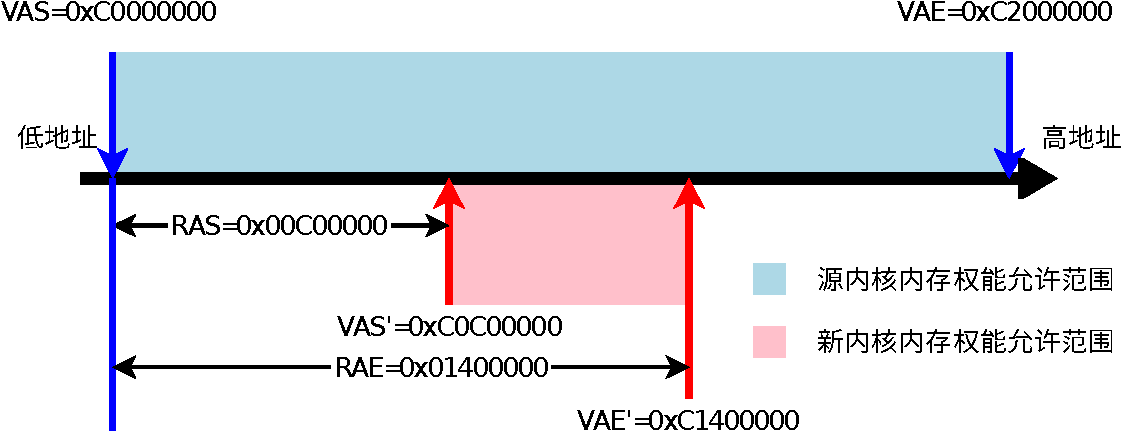
\includegraphics[width=0.72\textwidth]{Figure/image10.pdf}
    \caption{内核内存权能传递示例}
    \label{fig:3-3-kernel-memory-capability-transfer-example}
\end{figure}

此外，内核内存权能的上限值\footnote{也即内核结束绝对虚拟地址}不包括自身。在上例中，0xC1400000是不包括在新内核内存权能可操作的合法地址之内的，也即实际上允许的内核内存范围是0xC0C00000-0xC13FFFFF。上限必须大于下限，否则会返回错误。上限和下限在传入时都会被掩蔽后六位，对齐到64字节。如果内核内存登记表被配置为使用比64字节更大的槽位，那么内核会自动将传入的下限向上取整，上限向下取整，对齐到槽位大小。

本系统调用的可能返回值和一般的RME\_SVC\_CPT\_ADD操作完全一致，请参见\ref{subsec:2-transfer-a-capability}
。

\section{本章参考文献}\label{sec:3-chapter-bibliography}

\protect\phantomsection\label{cite:3-1}
{[}1{]}
Q. Wang, Y. Ren, M. Scaperoth, and G. Parmer, "Speck: A kernel for
scalable predictability," in Real-Time and Embedded Technology and
Applications Symposium (RTAS), 2015 IEEE, 2015, pp. 121-132.

\protect\phantomsection\label{cite:3-2}
{[}2{]} Emcraft Systems. uCLinux(2017).
\url{https://github.com/EmcraftSystems/linux-emcraft}

\protect\phantomsection\label{cite:3-3}
{[}3{]} G. Klein, K. Elphinstone, G. Heiser, J. Andronick, D. Cock, P.
Derrin, et al., "seL4: formal verification of an OS kernel," presented
at the Proceedings of the ACM SIGOPS 22nd symposium on Operating systems
principles, Big Sky, Montana, USA, 2009.

\protect\phantomsection\label{cite:3-4}
{[}4{]} Fiasco.OC website (2017).
\url{http://os.inf.tu-dresden.de/fiasco}

